\documentclass[10pt, a4paper]{article}
\usepackage{sectsty}
\sectionfont{\fontsize{12}{15}\selectfont}
\usepackage{indentfirst}
\setlength{\parindent}{0 em} \setlength{\parskip}{1 em} \renewcommand{\baselinestretch}{1} %\usepackage{mathptmx}\usepackage[scaled=0.91]{helvet} \usepackage{newtxmath}
\usepackage{newtxtext}
\usepackage{courier}
\usepackage{etoolbox}
\makeatletter
% \patchcmd{<cmd>}{<search>}{<replace>}{<success>}{<failure>}
\patchcmd{\@makechapterhead}{\huge}{\large}{}{}% for \chapter
\patchcmd{\@makechapterhead}{\Huge}{\large}{}{}% for \chapter
\patchcmd{\@makeschapterhead}{\Huge}{\large}{}{}% for \chapter*
\makeatother
% title center
\usepackage{titling}
\renewcommand\maketitlehooka{\null\mbox{}\vfill}
\renewcommand\maketitlehookd{\vfill\null}

%\usepackage{verbatim}
\renewcommand{\familydefault}{\sfdefault}
\usepackage[T1]{fontenc}
\usepackage[utf8]{inputenc}
%\usepackage{lmodern}
\usepackage[margin=1in]{geometry}
\usepackage[english]{babel}
\usepackage{csquotes}
\usepackage{graphicx}
\usepackage[notes,backend=biber]{biblatex-chicago}
\addbibresource{cite.bib}
\nocite{net-metering}
\nocite{market-price}
\nocite{scap-value}
\usepackage{float}
\usepackage{caption} % setting table 
\captionsetup[table]{position=bottom} % setting table
\usepackage[affil-it]{authblk}
\restylefloat{figure}
\usepackage{lipsum}
\usepackage{titlesec}
\titlespacing{\section}{0pt}{\parskip}{-\parskip}
\titlespacing{\subsection}{0pt}{\parskip}{-\parskip}
\titlespacing{\subsubsection}{0pt}{\parskip}{-\parskip}
\usepackage{fancyhdr}
\renewcommand{\headrulewidth}{0pt}
\usepackage[some]{background}
\SetBgScale{1}
\SetBgContents{\parbox{10cm}{%
\Huge \today\\[14cm]\rotatebox{180}{\Huge Internal Use Only}}}
\SetBgColor{gray}
\SetBgAngle{270}
\SetBgOpacity{0.2}

\begin{document}
\BgThispage
\pagestyle{fancy}
\title{\LARGE\bf{ Sensors Stations bi-weekly Report}}
\author{\large\bf{An Pham}}
\affil{\large\textup{California State Polytechnic University, Pomona}}

\maketitle
\newpage
\section*{\centering Abstract}
\fancyhf{}
\fancyhead[L]{Pham}
\fancyfoot[R]{\thepage}
\vspace{0 em}
% Describe the problem and why this problem is important
\normalsize
% What alternatives did you consider and why


% Your final suggestion and evaluation
% Things that remain to be done for this project to be fully complete
\par Due to the new sensors requirments and cost constrained, a new proposal is written to resolve part of challenges that the previous system exist.

\par Previous challenges was unable to unable to gather moisture data from the garden. Incompatibility when using rasperry pi as add-on sensors for the new system. Risks of inconsistency of dataset due to downtime of the station. Real-time data is limited because weewx service and cloud integration is seperated and shipped as different components. Database team has the success of organizing dataset with different timestamp.

% Your final suggestion and evaluation
\par To this end, having both Davis Weather Station and ECOWITT wireless gateway will help to add moisture sensors data. 

%\par \textbf{Keywords}:  (PW); Energy Storage; Southern California Edison {SCE}; Sensitivity Analysis; Before Tax Cash Flow (BTCF); After tax cash flow (ATCF); Straight Line Depreciation (SLD).
\newpage


\section{Client Requirement} %<2
% Ultimate goal of your client
\par This is a draft for new combination of previous Davis Weather Station and ECOWITT sensors gateway. As mentioned before, the goal is to maximize the values that the sensors station can provide. Values of the sensors such as rainfall, wind, temp, humidity, moisture, and barometer will be served as input for the project. However, this values  will rely Features of apps would be provided. Ideally, the goal of the project is to reduce complexity and number of components and maximize the values of t he sensors data. The consistency of dataset uploading will affect the integrity of the apps.  

\par Additionally, the begin time of the data have to be decided for sensors to compute. This assure the tracebility of the dataset.
% Consumer service goals and requirements that impact your analysis

% Demand (prediction of sales) estimation

\par Like any other IoT Projects, what we tries to deliver has the constraints of the project cost, schedule, and scope. If we decide to have increase dataset volume and deliverable as soon as possible. This lock us in the features that the vendor provided, and customization is limited. 

\noindent

\section{System Constraints} %<1
% Available Alternatives
\par This project was previously rely on 4G LTE network, which incurring costs of the stations in the long term. To be nimble of about the project, wifi was recommended as alternatives to bring down the cost of internet connection of IoT devices.
\par As side note, this 4G LTE Device has wifi capability.

\par To maintain the security of devices the only format is sent to the cloud is JSON. Since this is an IoT project, mqtt protocol will be used to send the message subscription model.


\begin{table}[!ht]
    \centering
    \caption{Operating Cost to Support 1 weather station with 4G lte}
    \begin{tabular}{|l|l|l|}
    \hline
    ~  & \textbf{Cost} & \textbf{Interval} \\ \hline
        \textbf{Internet Cost} & \$30 & Monthly \\ \hline
        \textbf{Cloud Cost } & \$45 & Monthly \\ \hline
    \end{tabular}
\end{table}
% Set the stage for the next section (economic model)
\section{Sensors  Development} %<2
% Development of cash flows for alternatives
\subsection{Integrate Raspberry Pi as Add-on sensors}
 \begin{figure}[!ht]
  \centering
    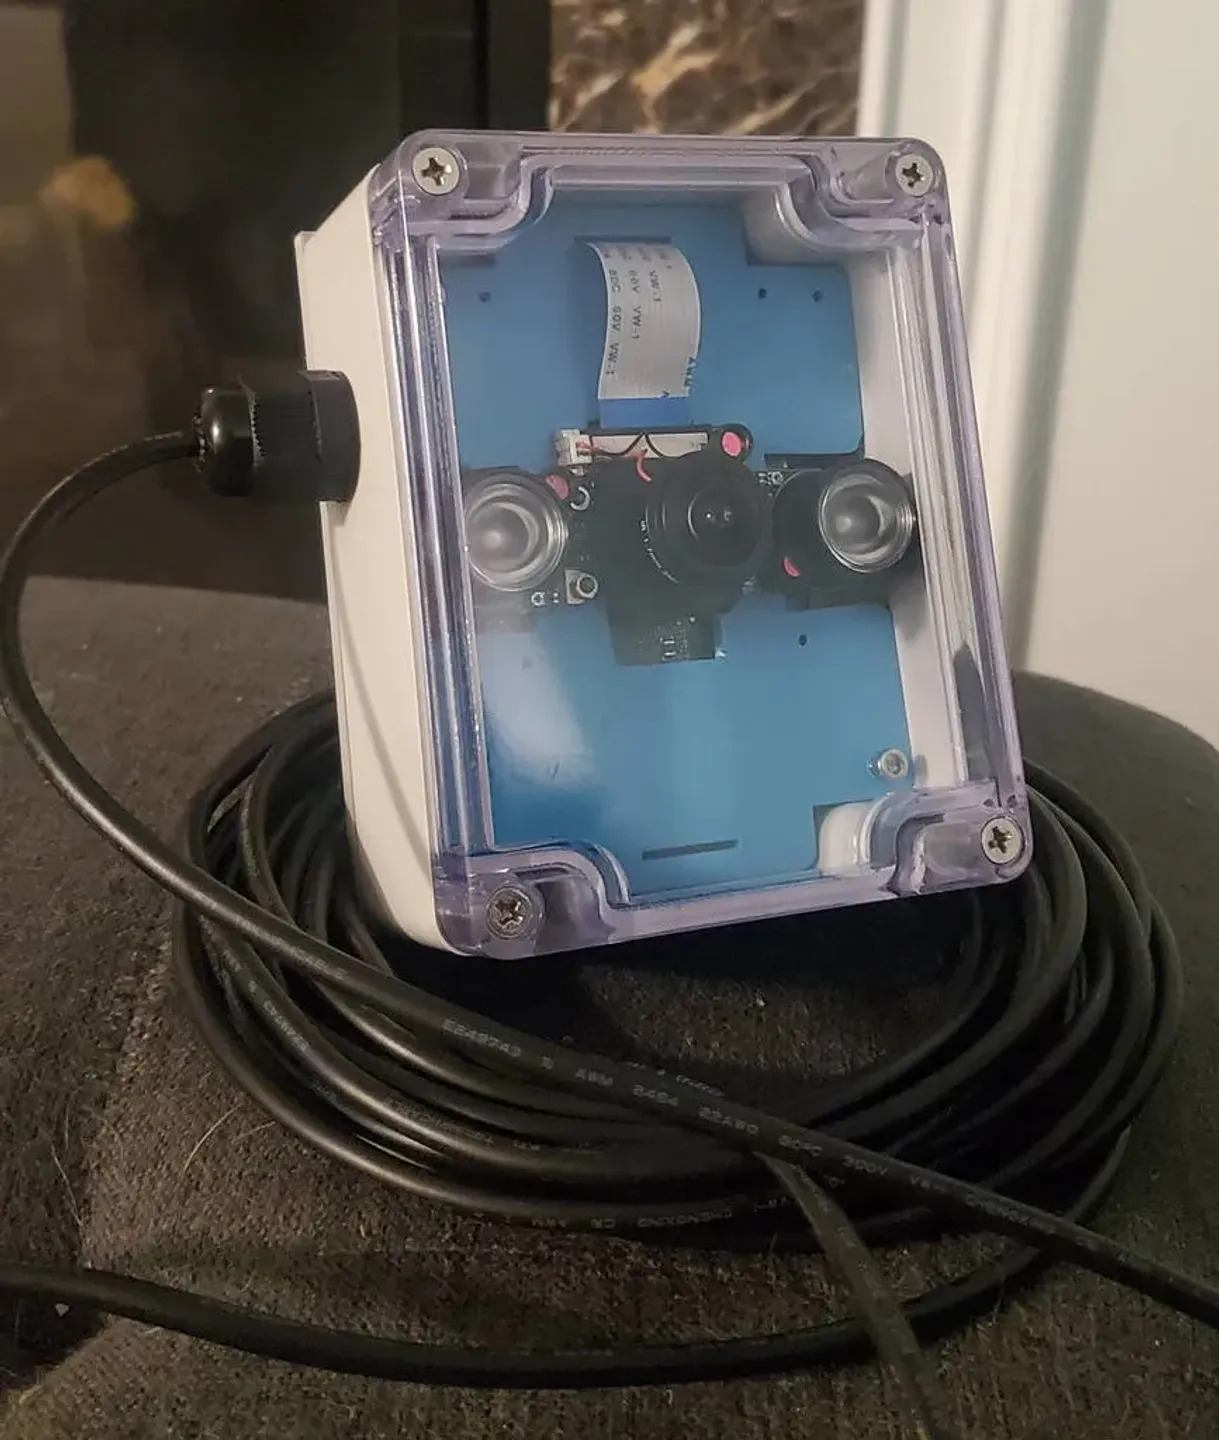
\includegraphics[width=5cm, height=5cm]{pi-encloser.jpg}
  \caption{Raspberry Pi based Sensor}
\end{figure}

 \begin{figure}[!ht]
  \centering
    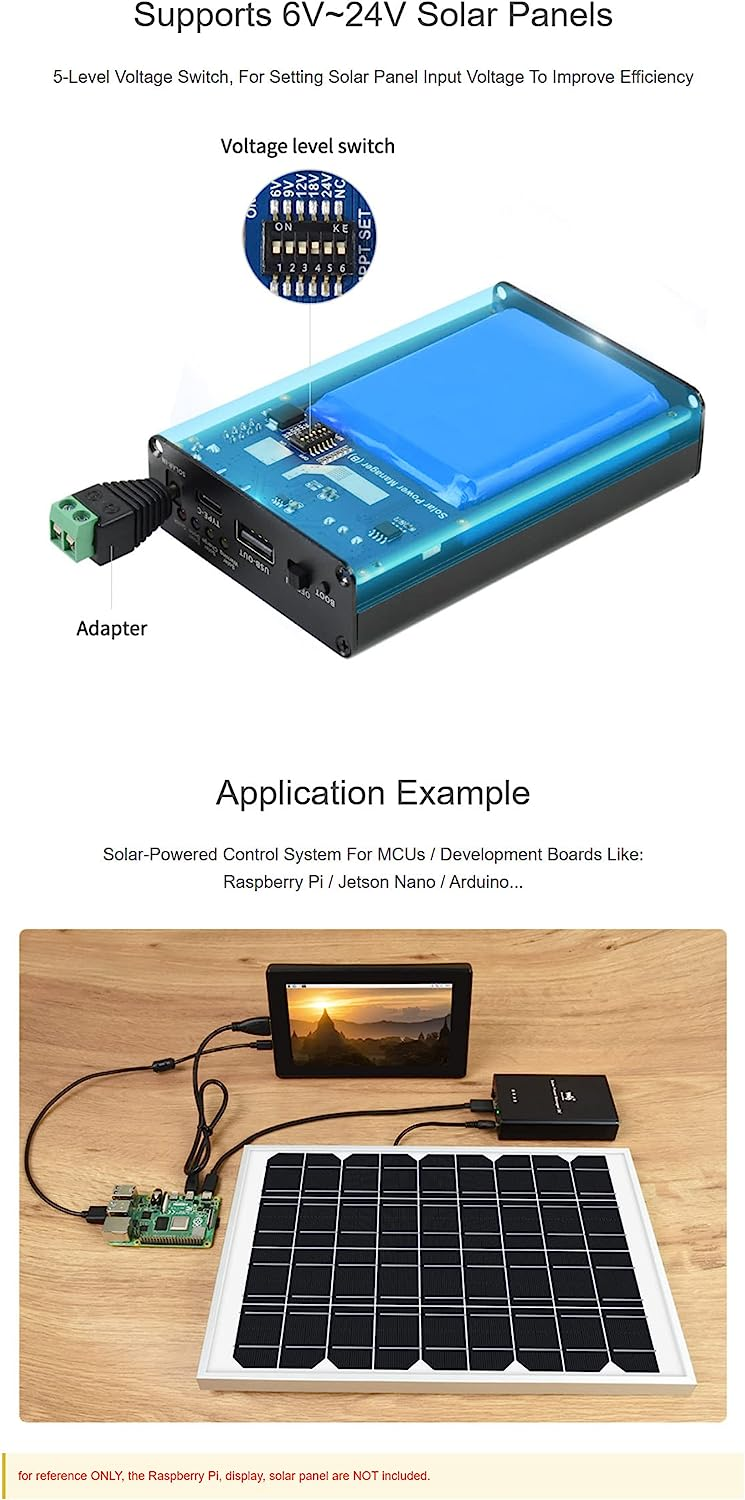
\includegraphics[width=10cm, height=10cm]{mppt-with-batter.jpg}
  \caption{Raspberry Pi Sensors with required component}
\end{figure}
 \begin{figure}[!ht]
  \centering
    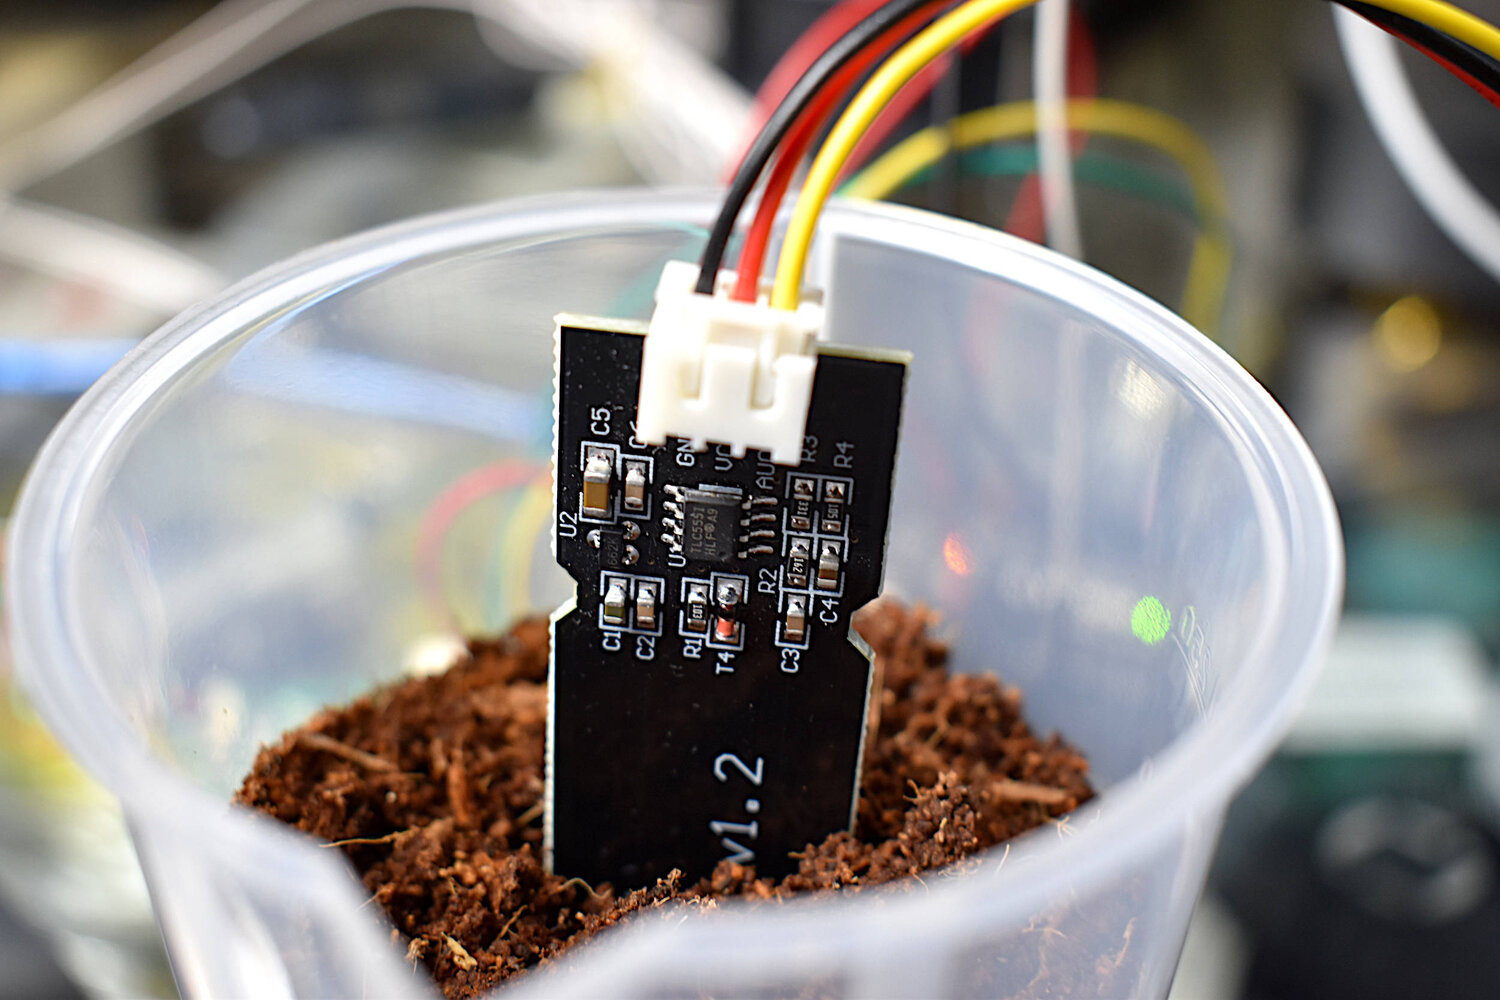
\includegraphics[width=10cm, height=5cm]{capacitive-moisture-sensors.JPG}
  \caption{Raspberry Pi Soil Moisture Sensor}
\end{figure}
\newpage
\par The use of raspberry pi as sensors node which is deployed in the garden. The parts are accessible and supported by the community. Housing of the raspberry pi is required. This the the continue work of Melvin since he had some python code to operate the sensors. But, the sensors are only able to operate indoor enviroment such as green houses. Therefore, all the component need water sealant. 
\par Steps to build the sensors.
\begin{enumerate}
  \item Submit the interfaces part.
  \item Prepare the junction box.
  \item Trim and grimp the wire.
  \item Drilling for wire accessibility.
  \item Test Mini Solar Station.

\end{enumerate}
\par Table below reflect the cost to build such sensor.
\begin{table}[!ht]
    \centering
    \begin{tabular}{|l|l|l|}
    \hline
    \textbf{Part Name} & \textbf{Description} & \textbf{Cost} \\ \hline
        \textbf{Junction Box} & Housing Raspberry Pi & \$28.39 \\ \hline
        \textbf{MPPT solar part} & Solar Power Management Module for 6V~24V Solar Panel & \$14 \\ \hline
	\textbf{Solar Panel} & ECO-WORTHY 12V Solar Panel 10W & \$28.94 \\ \hline
	\textbf{Capacitive Moisture Sensors} & Moisture sensors for Raspberry pi  & \$11.99 \\ \hline
	\textbf{Water Sealant} & Waterproof the moisture sensors & \$17.97 \\ \hline
	\textbf{Total cost} & - & \$101.26 \\ \hline 
    \end{tabular}
    \caption{Cost of building Raspberry Pi Sensors}
\end{table}

\par Addtionally, while having this raspberry pi sensor installed, we can add pump control for the irrigration system.
\begin{figure}[!ht]
  \centering
    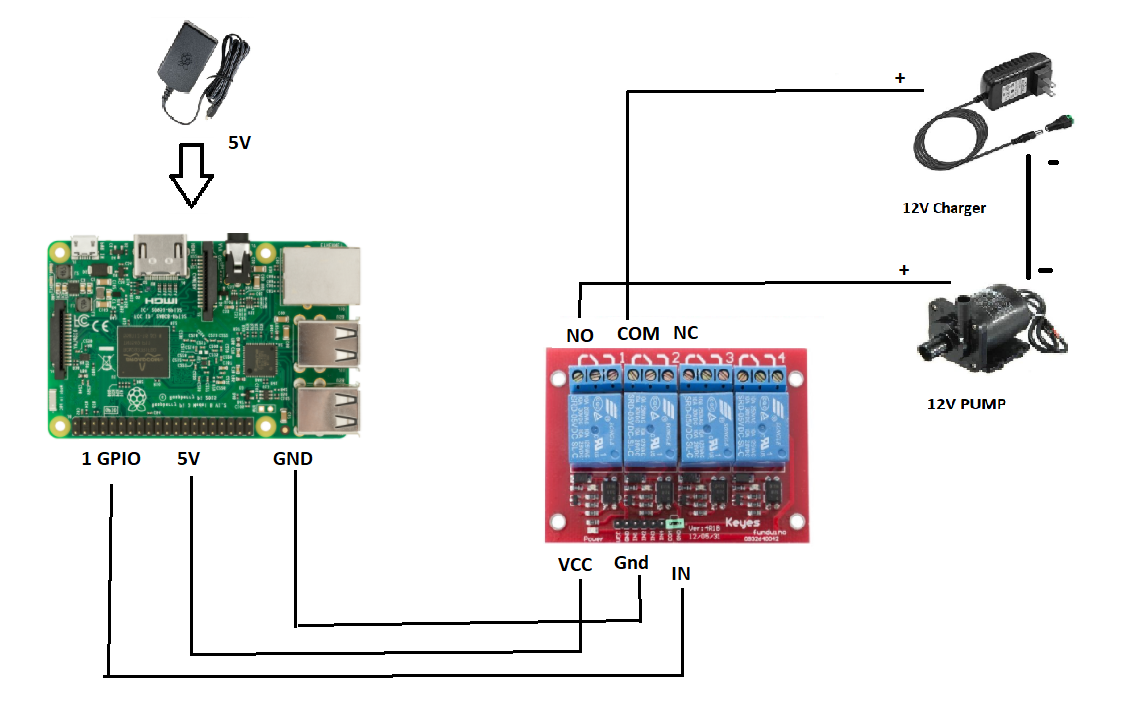
\includegraphics[width=1\textwidth, height=10cm]{water-pump.png}
  \caption{12V pump control with Raspberry Pi 4}
\end{figure}



\newpage
\subsection{Davis Soil Moisture Sensor}
\begin{figure}[!ht]
  \centering
    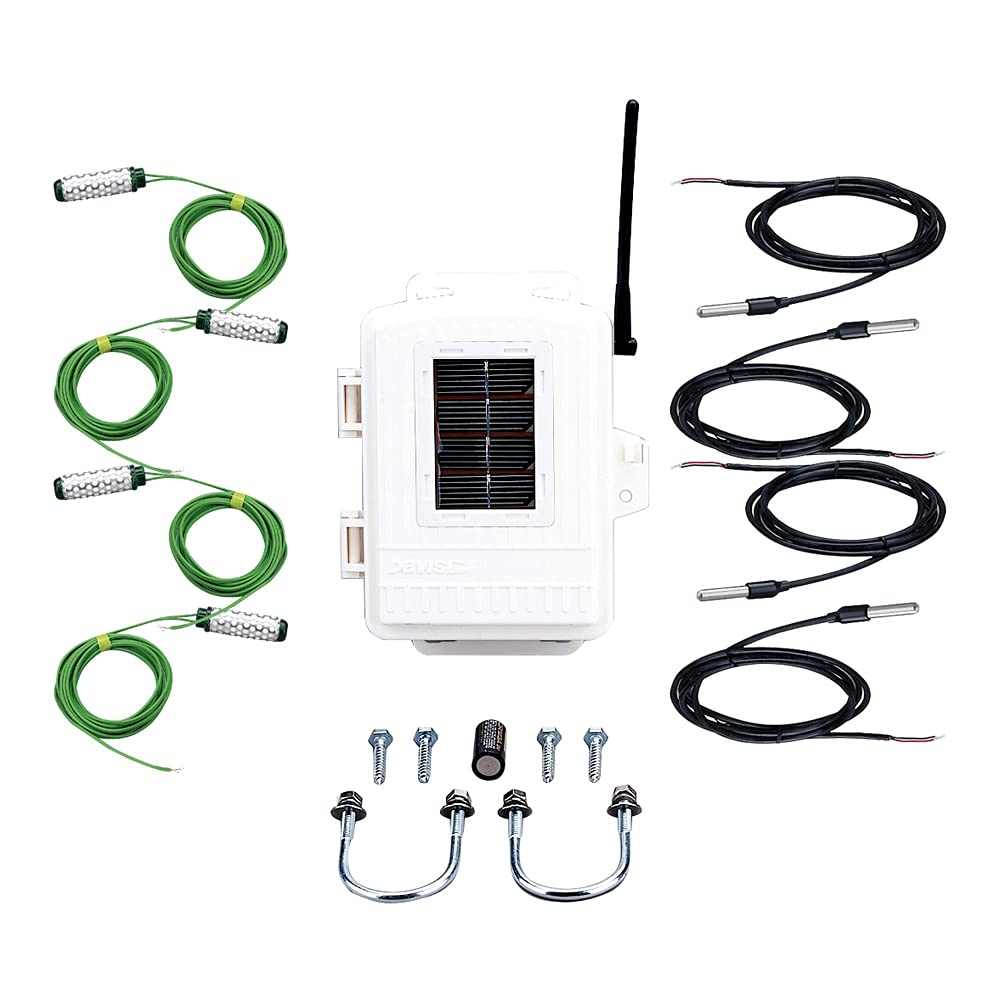
\includegraphics[width=1\textwidth, height=10cm]{davis-soil-moisture.jpg}
  \caption{Davis Soil Moisture and Leafwetness Sensor kit}
\end{figure}

\par This soil moitsture require the upgrade of new Davis Envoy Box from wire to wireless version.
\begin{figure}[!ht]
  \centering
    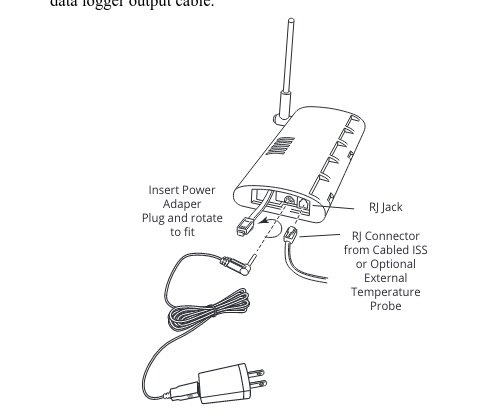
\includegraphics[width=\textwidth, height=5cm]{davis-envoy.jpg}
  \caption{Davis Wireless ISS Transmitter}
\end{figure}

\begin{table}[!ht]
    \centering
    \begin{tabular}{|l|l|l|}
    \hline
    \textbf{Part Name} & \textbf{Description} & \textbf{Cost} \\ \hline
        \textbf{Davis Soil Moisture and Leafwetness Sensor Kit} & Sensors hub for leaf sensors and soil sensor & \$637.27 \\ \hline
        \textbf{Davis Wireless Envoy} & Receiver for soil sensors stations & \$189.77 \\ \hline
	\textbf{Total cost} & - & \$827.04 \\ \hline 
    \end{tabular}
    \caption{Cost of building Raspberry Pi Sensors}
\end{table}


\par Since the whole sensor system is relied on Davis Weather Station, only one raspberry pi needed to deploy as only one database is stored and distribute to the dynamoDB cloud service.
\newpage
\subsection{ECOWITT Moisture Sensor}
\begin{figure}[!ht]
  \centering
    
\includegraphics[width=5cm, height=5cm]{ecowittsensors.jpg}
  \caption{ECOWITT Moiture Sensor Kit}
\end{figure}

\begin{figure}[!ht]
  \centering
    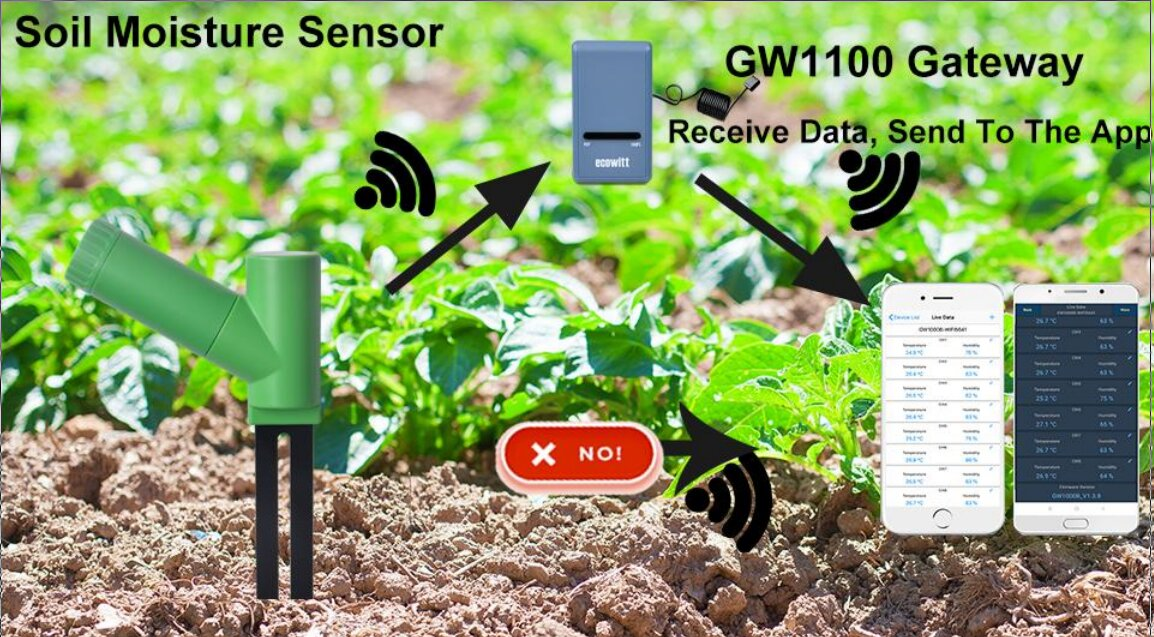
\includegraphics[width=5cm, height=5cm]{ecowittgw.jpg}
  \caption{ECOWITT Moiture Sensor with wireless gateway (GW1100)}
\end{figure}

\par Specification of device:
\begin{itemize}
\item This is wireless soil moisture sensors that collect moisture data within 72 seconds with inserted to the soil.
\item The sensors support real tiem data.
\item Reporting distance is within 300feet/100m(in open area).
\item  This sensors is powered by  AA” battery (not included, lithium recommended).
\item Battery change (Lithium) every 50 day.
\item  IP66 water resistant rated.

\end{itemize}
\paragraph{Installation: This devices will be installed with weewx as main software to archive the sensor data.}

\par The Wi-Fi gateway( GW1000/GW1100 ) can support max 8 soil moisture sensors. Each new sensor will be recognized as a new channel according to the Power-on sequence.
\par Please do not touch the stone or hard rock soil. If the soil is too hard and dry, it is possible to damage the sensor.
\par In order to work, this require two raspberry pis having weewx installed. Thus, there are two seperate database file exits on the pis.
\par The cost is \$53 for both wifi gateway (GW1100) and moisture sensors. We can also add uv sensors kit for extra \$62.97.
\begin{figure}[!ht]
  \centering
    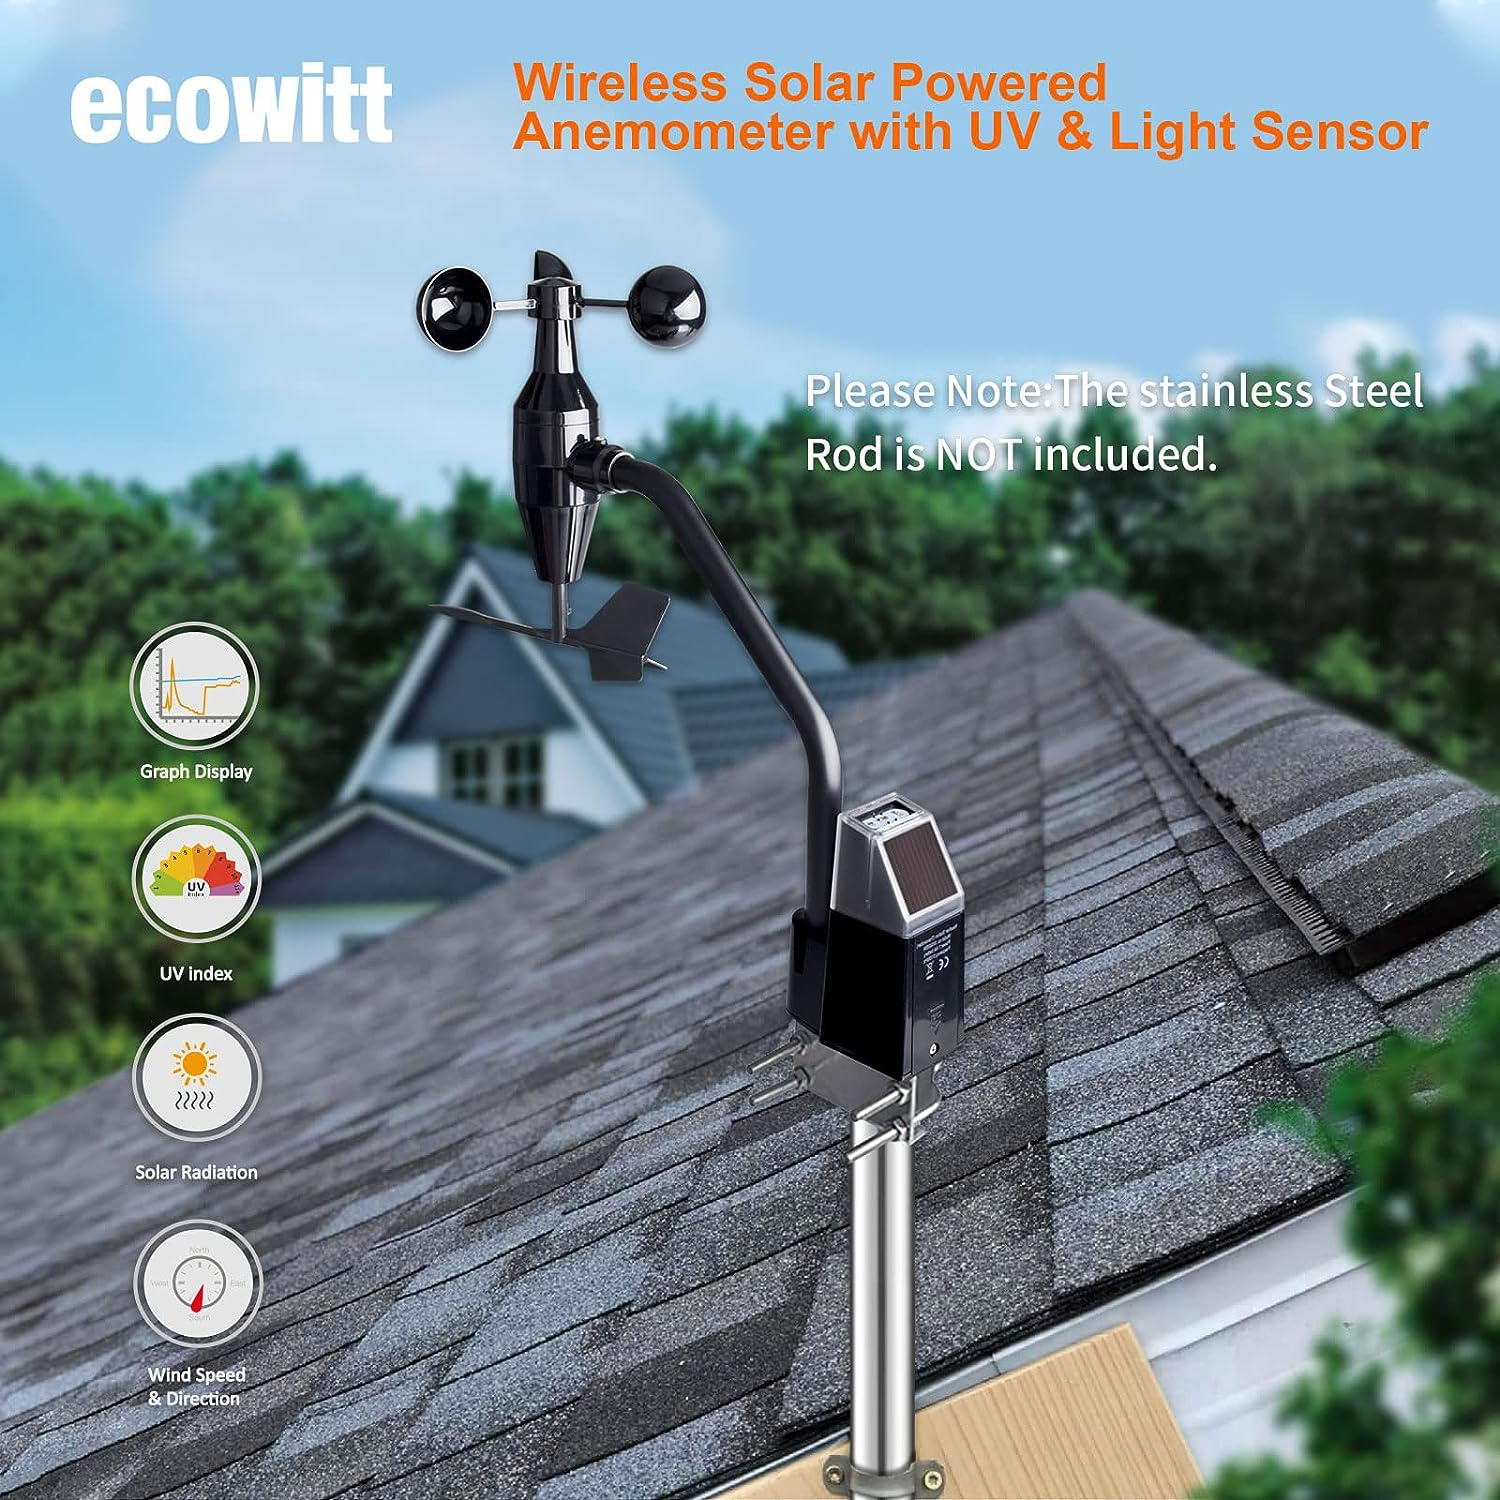
\includegraphics[width=5cm, height=5cm]{ecowitt-uv.jpg}
  \caption{ECOWITT UV and Light Sensor with wireless gateway (GW1100)}
\caption{ECOWITT Moiture Sensor with wireless gateway (GW1100)}
\end{figure}

\newpage
\section{Sensor Break-down Analysis} %<3
\begin{table}[!ht]
    \centering
    \resizebox{\columnwidth}{!}{%
    \begin{tabular}{|l|l|l|l|}
    \hline
	  & \textbf{Raspberry pi add-on} & \textbf{Ecowitt soil sensors} & \textbf{Davis Wireless sensors} \\ \hline
        \textbf{Solar required } & Yes & No & No (solar built-in)   \\ \hline
        \textbf{Battery required} & Yes & Yes (AA battery) & No \\ \hline
        \textbf{Weewx compatible} & No & Yes & Yes  \\ \hline
        \textbf{Back-up database} & optional & Yes & Yes \\ \hline
        \textbf{Cost} & \$101.26 & \$53 & \$827.04 \\ \hline
    \end{tabular}
  }
    \caption{Sensors Comparison}
\end{table}




\newpage

\section{Recommendation} %<2
% What should your client do?

% Why should they invest in that alternative?

\par After evaluating multiple solution, the compatibility of weewx is also a main requirement since they provide a backup local database.The assertation was made is to have both ECOWITT and Davis Weather Station running.
\par Decide the time frame for database to begin.
\begin{figure}[!ht]
  \centering
    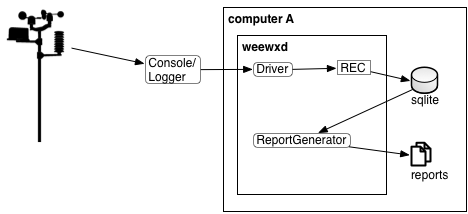
\includegraphics[width=\textwidth, height=5cm]{weewx-data-logger.png}
  \caption{Weex Data Logging}
\end{figure}




% information, etc.

\section{Inspection Instruction}

\begin{table}[!ht]
    \centering
    \begin{tabular}{|l|l|l|}
    \hline
    \textbf{Item Name} & \textbf{Tasks} & \textbf{Status} \\ \hline
        \textbf{Terminal or Bus Bar} & Check if the ciruit is closed or openned & - \\ \hline
        \textbf{MCB for solar controller} & Test for continunity of solar and battery charging  &  \\ \hline
        \textbf{Battery Charging Voltage} & Check if the mppt overcharge the battery & - \\ \hline
        \textbf{Drill Hole for Solar junction box} & Check if solar connector is waterproof  & - \\ \hline
    \end{tabular}
    \caption{Solar System Inspection Form}
\end{table}


% \input{appendix}

\end{document}
